\documentclass[12pt,oneside]{book}

\usepackage{times}
\normalfont
\usepackage[T1]{fontenc}
\usepackage{graphicx}
\usepackage{verbatim}

\begin{document}
\title{\textsc{Becca} version 0.4.0 \\User's Manual}
\author{Brandon Rohrer}

\maketitle
\tableofcontents
\newpage

% Skip an extra line between paragraphs
\addtolength{\parskip}{\baselineskip}

% List only chapters in the table of contents
\setcounter{tocdepth}{0}

\chapter{Get and run \textsc{Becca}}

Each chapter in this guide is designed to help you do something specific with \textsc{Becca}. This chapter helps you to get a copy of it on your local machine and run it on some generic worlds.

\section{Where do I get the code?}

You can download \textsc{Becca} from 

\texttt{www.openbecca.org} 

or 

\texttt{www.sandia.gov/rohrer} 

Or you can get the latest bleeding edge version (for which any of this documentation may already be outdated) from the github repository at

\texttt{https://github.com/matt2000/becca}.

\section{What tools do I need to run it?}

\textsc{Becca} is intended to be runnable on any hardware platform. This version relies on and was developed on 
\begin{itemize}
\item{Python 2.7}
\item{NumPy 1.6.1\footnote{The code makes use of at least one NumPy call, \texttt{count\_nonzero()}, that is not supported in NumPy 1.5.x.} }
\item{matplotlib 1.2}.
\end{itemize}
\textsc{Becca} has been run several different platforms (Mac OS 10.6.8, Ubuntu 12.04,\footnote{From developer SeH: \textsc{Becca}'s dependency on NumPy 1.6 is provided by the latest Ubuntu 12.04 package (but not Ubuntu 11.10 which provides NumPy 1.5).  Matplotlib is also provided, so everything seems to work fine on Ubuntu 12.04.} 32-bit Windows Vista, and 32-bit Windows 7) and IDEs/editors (Eclipse, PyScripter, IDLE, Stani's Python Editor, emacs, command line)\footnote{Any notes on successes or incompatibilities would be very welcome at \texttt{openbecca.org}.}. 

\section{How do I run it?}

Run \texttt{benchmark.py} in your Python interpreter. The \texttt{benchmark.py} module automatically runs \textsc{Becca} on a collections of worlds that are included with the download. It gives a report of \textsc{Becca}'s performance in the worlds. The benchmark can be used both to compare \textsc{Becca}'s speed on different computing platforms and, more importantly, to compare different variants of \textsc{Becca} against each other.

The worlds in \texttt{benchmark.py} are designed to be simple tests of \textsc{Becca}'s fundamental learning capabilities. \textsc{Becca} is an agent, in the sense that it makes decisions in order to achieve a goal, but it was created to be used in many different settings. The worlds tested in \texttt{benchmark.py} include one and two dimensional grid worlds and one and two dimensional visual worlds. The reward provided by each world gives motivation to \textsc{Becca} to behave in certain ways. When it behaves correctly, it maximizes its reward. This is \textsc{Becca}'s one and only goal. Each world in the benchmark provides periodic updates and final reports of its progress. 

Nice job. Now for the fun part.

\chapter{Write and run your first world}

This chapter steps you through the writing and running of your first world. In the process it explains \textsc{Becca}'s structure at a high level.

\section{What is a world?}

A \textsc{Becca} {\em agent} is a thing that chooses actions. In order for those actions to have any effect, they must be coupled to a {\em world}, an external environment that the agent can interact with. The agent--world configuration that \textsc{Becca} uses is shown in Figure~\ref{agent_world}. It is the canonical statement of the reinforcement learning problem: a reinforcement learning agent tries to choose actions so as to maximize the reward it receives.~\cite{sutton98} 

\begin{figure}
\centering
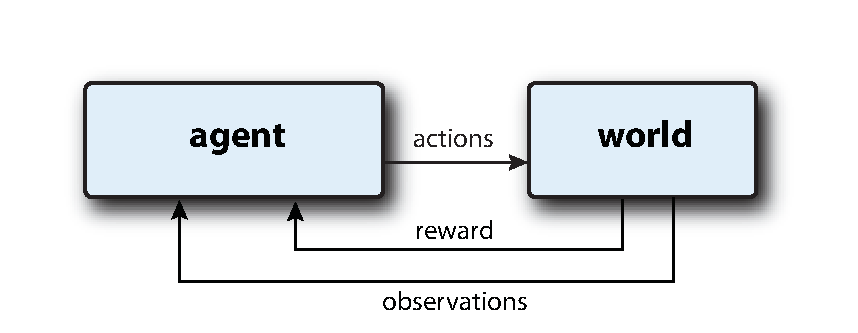
\includegraphics[height=5.0cm]{figs/agent_world.eps}
\caption{The agent-world coupling in \textsc{Becca}. The agent selects actions to execute on the world, which in turn provides observations and reward feedback.}
\label{agent_world}
\end{figure}

The architecture is modular. You can develop and run your own worlds without having to know very much about how the \textsc{Becca} agent works. The only constraints \textsc{Becca} imposes on worlds are:

\begin{itemize}
\item{A world must read in a fixed number of actions at each time step. This number is chosen by and defined in the world.}
\item{A world must provide a fixed number of sensory observations at each time step. This number is also chosen by and defined in the world.}
\item{A world must provide a scalar reward value at each time step.}
\item{All actions and observations are real valued, equal to 0, 1, or something in between.}
\item{The reward signal is real valued, equal to -1, 1, or something in between.}
\end{itemize}

Strictly speaking, \textsc{Becca} allows for two classes of observations, {\em sensors} and {\em primitives}. The only difference between the two is that the agent has to build sensors into features before it can use them, whereas it can use primitives as features immediately. Typically, observations that are likely to need some refining before they become useful (such as sets of pixel values) are passed in as sensors, and information that is more immediately useful (such as a contact sensor) are passed in as primitives. 

\section{How do I make a {\em hello} world?}

The quick and dirty way to get started making your own world is to copy an existing one and modify it. This is especially effective if there already exists something roughly similar to what you want. That's the approach we'll use to make a hello world.

\begin{enumerate}
\item{Save \texttt{worlds/grid\_1D.py} as \texttt{worlds/hello.py}}
\item{Replace the body of \texttt{step()} with this:
\begin{verbatim}
self.timestep += 1 
print self.timestep, ' hellos!'

sensors = np.zeros(self.num_sensors)
primitives = np.zeros(self.num_primitives)
reward = 0
return sensors, primitives, reward
\end{verbatim}
and save the changes.
}
\item{Add the line 
\begin{verbatim}
from worlds.hello import World
\end{verbatim}
to \texttt{tester.py}. Make sure all the other lines beginning with \texttt{from worlds}...  are commented out.
}
\item{Run \texttt{tester.py}}
\end{enumerate}


\section{What do I need to implement in my world?}

\texttt{hello.py} runs because it meets a few basic requirements. This section lists them and describes the mechanics of a \textsc{Becca} world.

Any world needs to have at least these three publicly accessible member variables,

\begin{itemize}
\item{\texttt{num\_sensors}}
\item{\texttt{num\_primitives}}
\item{\texttt{num\_actions}}
\end{itemize}

these three methods,

\begin{itemize}
\item{\texttt{step()}}
\item{\texttt{is\_alive()}}
\item{\texttt{set\_agent\_parameters()}}
\end{itemize}

and perhaps two optional methods,

\begin{itemize}
\item{\texttt{is\_time\_to\_display()}}
\item{\texttt{vizualize\_feature\_set()}}
\end{itemize}

each of which are all described in more detail below.

\subsection{\texttt{num\_sensors}}
Specifies the number elements in the array of sensor information that is passed to the agent at each time step.

\subsection{\texttt{num\_primitives}}
Specifies the number elements in the array of feature primitives that is passed to the agent at each time step.

\subsection{\texttt{num\_actions}}
Specifies the number elements in the array of actions that it expects to receive from the agent at each time step. Together, these three variables define the interface between the agent and the world. They may be different for each world, but they must remain constant within a single world. \footnote{In this version of \textsc{Becca}, each of these variables must be at least 1. \textsc{Becca} doesn't yet know how to handle empty sensory or primitive arrays. Worlds that have no sensors or primitives can pass a single zero value at every time step to achieve this.}

\subsection{\texttt{step()}}
Advances the world by one time step. This is single most important method in a world. It defines how the world will respond to the agent. It accepts an array of actions and returns an array of sensors, an array of primitives, and a reward value. \textsc{Becca} places no constraints on the complexity or the execution time of the \texttt{step()} method. It can incrementally advance a simulation, pass and receive network packets, or provide an interface to physical robot. The agent will wait until \texttt{step()} finishes and returns its observation and reward information before advancing to the next time step.

\subsection{\texttt{is\_alive()}}
Informs the executing loop when to stop. The top level execution loop (as implemented in \texttt{benchmark.py} and \texttt{tester.py} continues to run \textsc{Becca} through its agent-world-agent cycle until \texttt{is\_alive()} returns false.

\subsection{\texttt{set\_agent\_parameters()}}
Sets the the agent's internal parameters to values specific to the world. \textsc{Becca} has a quite a few constants that affect its operation, in the neoghborhood of 20 at last count. Most of these are set to values that seem to work for all worlds in the benchmark battery. But for development and troubleshooting, it has proven useful to be able to adjust some of \textsc{Becca}'s parameters manually. It is my hope that, in time, a single set of parameters will prove generally useful across a broad set of tasks. In the meantime this method provides a mechanism for world-specific knob-twiddling.

\subsection{\texttt{is\_time\_to\_display()}}
Informs the executing loop when to display the feature set by returning \texttt{True}. This is for visualization purposes only and doesn't help \textsc{Becca} learn in any way. This method is optional. If it doesn't exist, the execution loop just moves on.

\subsection{\texttt{vizualize\_feature\_set()}}
Displays the feature set when \texttt{is\_time\_to\_display()} returns \texttt{True}. The feature set is expressed in terms of sensors, primitives, and actions by the agent. This method takes those feature representations and interprets them for the user in terms of what it knows about how those signals. For instance, if the sensors correspond to pixel values from a camera, this method would render the sensor component of each feature as an image. The agent has no information about where its sensor and primitive arrays came from or about what its actions do in the world. This method lets the world give a world-specific interpretation of those values to the user.

Worlds of course may have any number of other member variables and methods for internal use. Others that have proven useful in the benchmark battery worlds include \texttt{calculate\_reward()} and \texttt{display()}.

\section{What is \texttt{base\_world.py}?}
``Wait a second," you say. ``My \texttt{hello.py} didn't have an \texttt{is\_alive()}, but you said it needed one. What's up with that?"

These two lines from the beginning of the module help to solve that mystery:
\begin{verbatim}
from .base_world import World as BaseWorld
class World(BaseWorld):
\end{verbatim}

\texttt{hello.py} is actually a subclass of \texttt{base\_world.py},\footnote{If terms like {\em class}, {\em subclass}, {\em inheritance}, and {\em override} aren't familiar to you in this context, I'd highly recommend doing some quick reading on object-oriented (OO) programming. The concepts aren't that tricky, but they are extremely useful when discussing OO software, such as \textsc{Becca}.} which defines a generic \texttt{is\_alive()}. It also defines a generic \texttt{set\_agent\_parameters()} and \texttt{step()}, as well as default values for  \texttt{num\_sensors}, \texttt{num\_primitives}, and \texttt{num\_actions}. When you subclass it to create a new world you, only need to override those methods and variables that you want to change.


\section{How do I run my world?}
\texttt{tester.py} is the vehicle for coupling a new world with a \textsc{Becca} agent and running them. You've already added your hello world to \texttt{tester.py} and run it. This section gives a line-by-line overview of the rest of the module and what it does. This will help make clear a few of the finer points of running a world.

\begin{enumerate}
\item
Import the relevant modules. In particular import a \texttt{World} class from a module containing one.
\begin{verbatim}
import numpy as np
from agent.agent import Agent
from agent import viz_utils
from worlds.hello import World
\end{verbatim}

\item
Define the \texttt{main} method and initialize some objects. When initializing the \texttt{agent}, there are two optional variables, \texttt{MAX\_NUM\_FEATURES} and \texttt{agent\_name}.  \texttt{MAX\_NUM\_FEATURES} provides an upper limit on the number of features that the agent can create and can be set appropriately to prevent \textsc{Becca} from using up all your RAM. \texttt{agent\_name} is a text string used to identify a specific agent and is useful if you are planning to save the agent or restore it from a previously saved agent. Note that if you do this, the world used in both cases must have the same number of sensors, primitives, and actions.
\begin{verbatim}
def main():
    
    world = World()
    
    agent_name = "test";
    MAX_NUM_FEATURES = 3000
    agent = Agent(world.num_sensors, 
                  world.num_primitives, 
                  world.num_actions, 
                  MAX_NUM_FEATURES, 
                  agent_name)

\end{verbatim}

\item
Restore the agent to a previously saved agent, if desired.
\begin{verbatim}
    #agent = agent.restore()
\end{verbatim}
    
\item
Modify the agent's parameters according to the requirements of this particular world. Initialize actions such that the first set of commands to the world is always zeros.
\begin{verbatim}
    world.set_agent_parameters(agent)
    actions = np.zeros(world.num_actions)
\end{verbatim}

\item
Begin the execution loop. Couple the output of the world into the input of the agent and vice versa.
\begin{verbatim}    
    while(world.is_alive()):
        sensors, primitives, reward = world.step(actions)
        actions = agent.step(sensors, primitives, reward)
\end{verbatim}

\item
If the necessary methods exist, and if they dictate, display the feature set to the user.        
\begin{verbatim}    
    try:
        if world.is_time_to_display():
            world.vizualize_feature_set(
                viz_utils.reduce_feature_set(
                agent.grouper), 
                save_eps=True)
            viz_utils.force_redraw()
    except AttributeError:
        pass
\end{verbatim}

\item
After the world has completed its lifetime, give a final report of the agent's performance.    
\begin{verbatim}    
    agent.report_performance()
    agent.show_reward_history()
    
    return
\end{verbatim}

\item
And finally, run \texttt{main()}    
\begin{verbatim}    
if __name__ == '__main__':
    main()
\end{verbatim}

\end{enumerate}

% TODO: flesh this out
%\section{Are there any tricks for making a world so that \textsc{Becca} can learn it?}
% binary-style inputs
% make sure Becca gets enough information--could a human solve the task?
% primitives--high-level sensors
% actions--high level vs. low level


\chapter{Share your world with other \textsc{Becca} users}
\label{world_share}

\textsc{Becca} was created so that it would be easy to use and share what you create with others. This section describes how to get your world out and get the word out.

\section{Where do I put my world module so that others  can find it?}

The most convenient place to share \textsc{Becca} content is GitHub. Open a GitHub account if you don't have one already, create a repository, and populate it with your world's code. 

The official \textsc{Becca} core code base is hosted on GitHub in one of Matt Chapman's repositories:

\texttt{https://github.com/matt2000/becca}

It contains a tagged version of this code, plus all the incremental commits that are working toward the next version. The core contains the full agent, plus a battery of worlds for benchmarking, and a couple of utility modules. The plan is to keep the \textsc{Becca} core small and trim with only the necessaries for getting a new user up and running. 

Contributed code and modifications will be available separately. The details for how this will happen are still taking shape as our community is still young and small, but for now contributed modules will be listed with brief descriptions on the \texttt{openbecca.org} site. This list will be as exhaustive as possible, until the volume of contributions forces us to find another way to do things.

\section{How do I tell them about it?}

If you didn't record it, it didn't happen. When you do something new, make a record of it in some way so you can show everybody how cool it is. There are lots of good ways:

\begin{itemize}
\item Make a video
\item Grab screenshots
\item Draw diagrams
\item Write an appendix to this users guide\footnote{If you're new to LaTeX, just copy one of the users guide chapter files and modify it to tell your story. The \texttt{.tex} files are in the \textsc{Becca} GitHub repository under \texttt{doc/user\_manual/}.}
\item Write a conference paper\footnote{I've had good luck with the Artificial General Intelligence (AGI) and Biologically Inspired Cognitive Architectures (BICA) conference series. Also the combined International Conference on Development and Learning/Epigenetic Robotics Conference (ICDL/EpiRob) is good and the brand new AAAI Spring Symposium on Integrating Artificial Intelligence looks to be fantastic.}
\item Write a paragraph.
\end{itemize}

Then, whatever form your documentation takes, share it around. Right now, the best way to broadcast notifications to other \textsc{Becca} users is to post in the Google Group, 

\begin{verbatim}
https://groups.google.com/forum/?fromgroups#!forum/becca_users
\end{verbatim}

Sign up if you haven't yet. Incidentally, subscribing to the group's posts is also the best way to hear about others' contributions to the body of \textsc{Becca} code.

This is subject to change. The preferred way to advertise new content may eventually migrate to an \texttt{openbecca.org} forum.



\chapter{Modify your agent code}

This section is to help you get started hacking your own version of the \textsc{Becca} agent. Don't be afraid to jump in and start rewiring it.

\section{How is the agent code structured?}

This section will give just an overview of the structure so that you have some idea about where to start making changes. The overall structure of \textsc{Becca} is shown in Figure~\ref{becca_block}. A thorough description is included in Appendices~\ref{perceiver_chapter} and~\ref{actor_chapter}. 

\begin{figure}
\centering
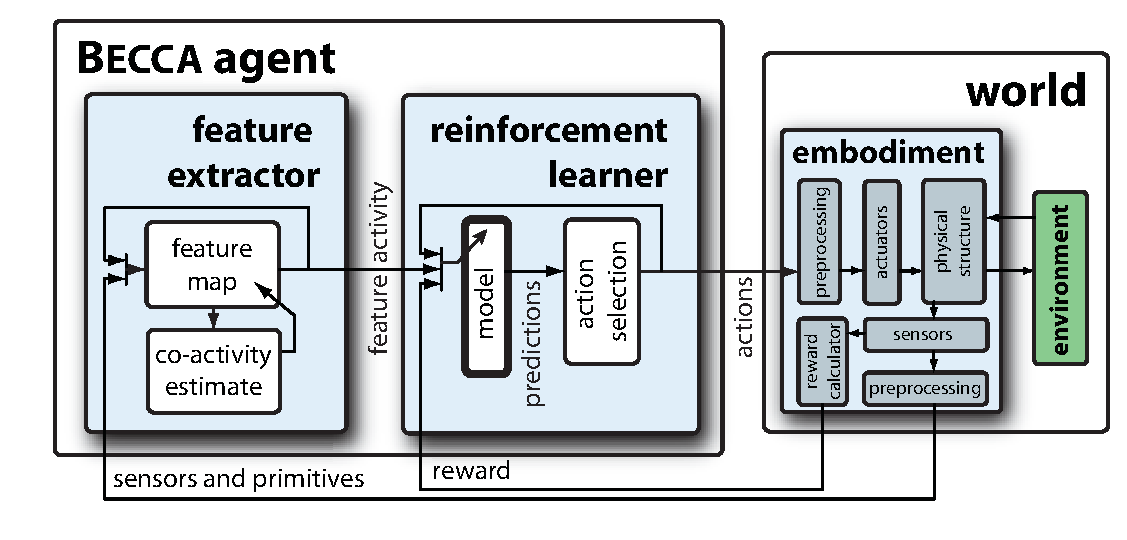
\includegraphics[height=6cm]{figs/becca_0.4.5_block.eps}
\caption{A high-level block diagram of how \textsc{Becca} is put together.}
\label{becca_block}
\end{figure}

The agent's functionality is contained in three main classes, corresponding to the blocks in Figure~\ref{becca_block}. The feature extractor is instantiated in the \texttt{perceiver} class, the reinforcement learner is instantiated in the \texttt{actor} class, and the \texttt{agent} class ties them together. 

\subsection{\texttt{Agent}}
\begin{itemize}
\item Performs executive functions, such as saving and reporting.
\item Calls \texttt{Perceiver.step()} and  \texttt{Actor.step()} at each time step.
\end{itemize}

\subsection{\texttt{Perceiver}}
\begin{itemize}
\item Forms inputs into features.
\item Determines which features are active at each time step.
\item Feeds those features back as additional inputs.
\end{itemize}

\subsection{\texttt{Actor}}
\begin{itemize}
\item Contains and maintains a library of \texttt{transition}s, each consisting of four states: a \texttt{context}, a \texttt{cause}, an \texttt{effect}, and an \texttt{effect\_uncertainty}.  \texttt{transition}s are conceptual only, and are not actually member variables.  States include the activity of primitives, features, and actions at a point in time are represented as a numpy array. 
\item Based on the \texttt{Agent}'s current state and history, chooses an action likely to bring reward.
\end{itemize}

\subsection{Utility modules: \texttt{utils} and \texttt{viz\_utils}}
\begin{itemize}
\item Performs general math chores. May be used by multiple classes.
\item Visualizes the internal states of classes for the user.
\end{itemize}

\section{Is my agent better than the core agent?}
The most natural question to ask after changing the agent is whether the new version is better than the old one.\footnote{This is also a natural question to ask of other reinforcement learning agents. If you care to, you can code up any RL agent in Python and test it against \textsc{Becca} on the benchmark. If you do, I'd be really curious to hear your results.} The answer will of course depend on what you mean by ``better". The choice of performance measure has a great deal of influence on the performance levels of individual agents. The only necessary characteristic of a performance measure is that it produce a numerical value when applied to an agent. If you have a specific performance measure in mind, code it up and use it. If not, consider \texttt{benchmark.py}. 

The worlds in \texttt{benchmark.py} are intended to be a testing battery that requires a broad learning capability to do well on. Admittedly, the battery members in this version of the benchmark are very basic. New worlds are added only when \textsc{Becca} can perform well on all the old ones, each new world has brought to light more of \textsc{Becca}'s bugs. This process is great for ironing out the kinks in \textsc{Becca}, but a little slow. As \textsc{Becca} matures, the worlds in the benchmarking battery will also grow in number and sophistication. Since the benchmark is likely to change with each release of \textsc{Becca}, the version number of each benchmark will be an important identifier.

The worlds in this version of the benchmark are described briefly below.

\subsection{\texttt{grid\_1D.py}}

\begin{figure}
\centering
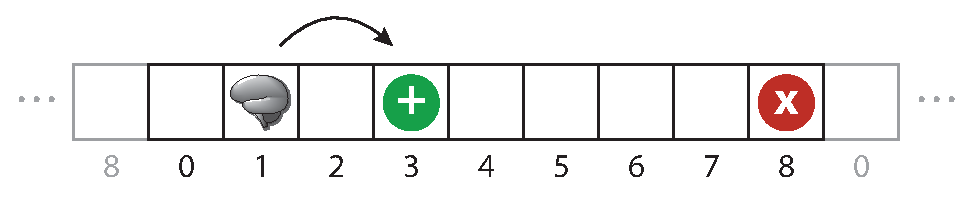
\includegraphics[height=2.5cm]{figs/grid_world_1D.eps}
\caption{The one-dimensional grid world.}
\label{grid_1D}
\end{figure}

As the name implies, this is a one-dimensional grid world. There are nine discrete states arrayed in a line, and the agent steps between them in increments of 1, 2, 3, or 4 steps in either direction. Stepping right from the rightmost state lands the agent in the leftmost state and vice versa, making the world into a ring. The fourth state from the left gives the agent a reward of 100 and the far right state inflicts a punishment (negative reward of -100). Every step the agent takes also incurs a cost of  1. This world was designed to be simple, yet non-trivial, and has proven very useful in troubleshooting \textsc{Becca}.

\subsection{\texttt{grid\_1D\_ms.py}}

The \texttt{ms} stands for `multi-step'. This world is identical to the \texttt{grid\_1D.py} world, except that the agent may only step in increments of one in either direction. Occasionally random perturbations place the agent in new positions and it must make its way back to its goal using multiple steps, rather than in a single step. This world requires multi-step planning and is a challenge for some learning agents. Right now \textsc{Becca} can only make its way directly back to the goal when it is within a couple of steps. It is waiting on better multi-step planning to perform really well on this task.

\subsection{\texttt{grid\_1D\_noise.py}}

The \texttt{noise} refers to the fact that the primitives reported by this world include a number of noise elements, whose values are randomly generated at each time step. It is similar to the  \texttt{grid\_1D.py} world, but has only three states.  The second of these gives a reward of 100, and the other two a punishment of -100. Many reinforcement learning algorithms do not have a mechanism for handling noise or irrelevant data and this world poses a challenge to them. 

\subsection{\texttt{grid\_2D.py}}

This is similar to \texttt{grid\_1D.py}, but extended to two dimensions, with 5 rows and 5 columns. Each dimension wraps around, similar to the one dimensional version. This gives the world a toroidal topology and makes it impossible to fall off of it or run into any walls. The agent can make steps of 1 or 2 columns or rows in any of the four compass directions. A location in the lower right portion of the world gives a reward of 100, and a second location in the upper left portion of the world gives a punishment of -100. And, as with the one dimensional world, every step incurs a cost of 1. The agent's position in the world is represented using an array of 25 primitives, one for each possible location. 

\begin{figure}
\centering
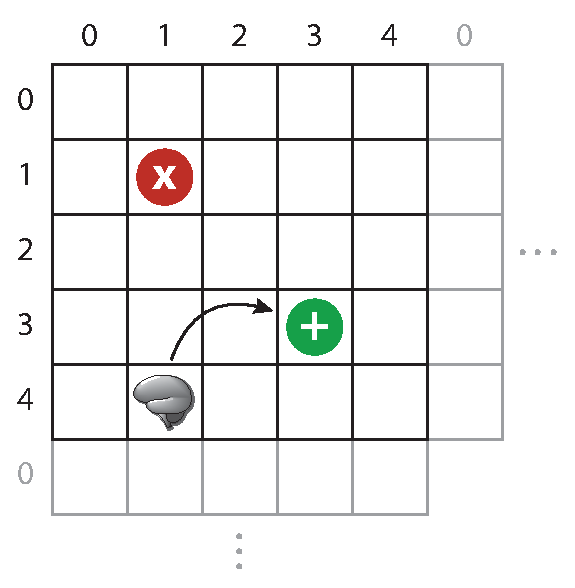
\includegraphics[height=10cm]{figs/grid_world_2D.eps}
\caption{The two-dimensional grid world.}
\label{grid_2D}
\end{figure}

\subsection{\texttt{grid\_2D\_dc.py}}

The \texttt{dc} stands for `decoupled' and refers to the fact that the column and row position of the agent are represented separately, each in an array of 5 primitive elements, giving this world a primitive array size of 10 rather than 25. This forces \textsc{Becca} to consider multiple inputs simultaneously when making decisions, making it a slightly more difficult world than \texttt{grid\_2D.py}.

\subsection{\texttt{image\_1D.py}}

The two major differences between the image worlds and the grid worlds are:

\begin{enumerate}
\item In the image worlds position is continuous, rather than discrete.
\item In the image worlds observations are arrays of sensors, rather than arrays of primitives.
\end{enumerate}

In the one dimensional case, the agent is looking at a mural (albeit a very boring one) and can shift its gaze right and left. It is rewarded for staring at the center of the mural.

The agent can move in increments of 1/4, 1/8, 1/16, and 1/32 of the mural width to both the right and left until it reaches the limits of the mural. All actions are also subject to an additional 10\% random noise. The agent's field of view is half as wide as the mural. The reward region is 1/16 as wide as the mural and positioned at its center. When the center of the agent's field of view falls within the reward region, the agent receives a reward of 100. Within its field of view, the agent averages pixel values in a 10 $\times$ 10 grid to create a coarsely pixelated version of the mural. Each coarse pixel can be between 0 (all black) and 1 (all white). The pixel values are passed through a center-surround filter, which calculates the extent to which each pixel value is lighter than or darker than its neighbors. The center-surround values are passed to the agent in a 100 element sensor array.

\begin{figure}
\centering
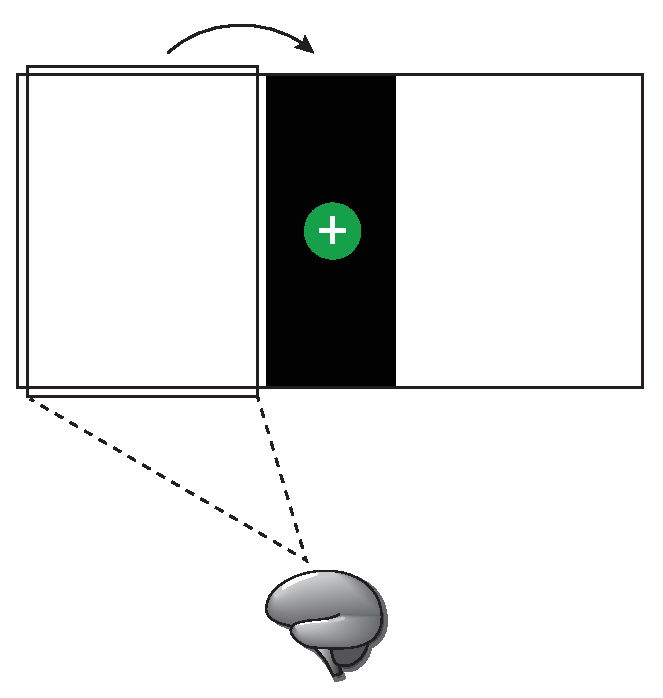
\includegraphics[height=8cm]{figs/image_world_1D.eps}
\caption{The one-dimensional image world.}
\label{image_1D}
\end{figure}

It's worth noting that a naive $\mathcal{Q}$-learning approach to this problem would require creating a $2^{103}$-element state table. The global information storage capacity is currently on the order of $2^{70}$ bytes.

\subsection{\texttt{image\_2D.py}}

This world is similar in many ways to the one dimensional version, just extended to a second dimension. In it, the agent must center its gaze both horizontally and vertically to receive the full reward. One difference is that it pixelizes its world into a 5 $\times$ 5 grid (resulting in a center-surround sensor array of 25 elements). A second difference is that the agent receives a reward of 50 if its gaze is centered horizontally and an additional reward of 50 if its gaze is centered vertically. 

\begin{figure}
\centering
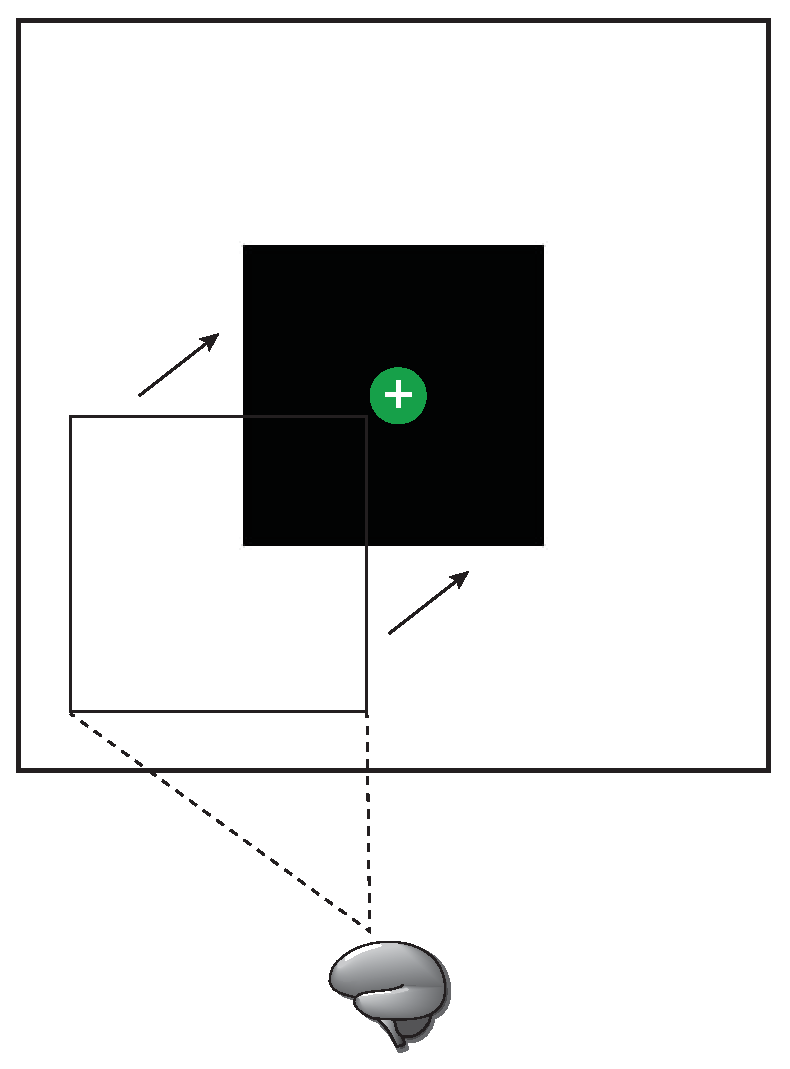
\includegraphics[height=12cm]{figs/image_world_2D.eps}
\caption{The two-dimensional image world.}
\label{image_2D}
\end{figure}

\subsection{\texttt{world\_utils.py}}

There are some jobs that crop up repeatedly in multiple worlds. This module is a common toolbox where functionality can be shared. So far this is limited to image processing functions, including center-difference filtering and visualizing features in image data.



\chapter{Share your agent with other \textsc{Becca} users}

So you've modified your agent, it's really cool, and now you want to share it. Everything in Chapter~\ref{world_share} about sharing your worlds applies to sharing agents too. Unlike other open source software projects, branching is not discouraged. The motivation behind \textsc{Becca} is not to produce a slick tool that can be used as a black box. It is to make an architecture that gets used as often and as widely as possible. 

To some extent every implementation will be custom. Ideally, every implementation will be driven by the well-articulated vision of one person or of a small group. \textsc{Becca} is intended to be a generic starting point for your work. If it were an ice cream flavor, it would be vanilla. It will be up to you to create chocolate, cappachino, and habanero. When you do, please pass them around so we can all get a taste.

If you have modifications, edits, or additions that you think may improve the core \textsc{Becca} code, send a GitHub pull request to Matt Chapman, the curator of the core repository. An informal discussion will ensue in the becca\_users group, and based on the outcome, your code will be incorporated into the core repository.

\section{How do I make my code look like the rest of the core?}
For any code destined for the repository, please follow these high level style goals (in rough order of priority):
\begin{enumerate}
\item Usability--a new user can apply it to their project with a minimum
of effort and pain
\item Readability--a new developer can get oriented in the code with a
minimum of effort and pain
\item Brevity--the number of packages, modules, methods, and lines of
code are minimized
\item Performance--it works well and quickly
\end{enumerate}

The implications of these priorities are that if performance can be increased by 0.2\% by importing another
package or adding another module, it's not worth it. But an
increase of 50\% would probably merit it. This may also mean neglecting
some code development best practices because of their verbosity.
Adding another layer of abstraction in places may make the core more
easily extensible, but that may not be worth making it harder to
navigate.

On low level style specifics, the PEP 8 Python style guide\footnote{\texttt{http://www.python.org/dev/peps/pep-0008/}} and PEP 257 Docstring style guide\footnote{\texttt{http://www.python.org/dev/peps/pep-0257/}} are the default word on style. However if there is ever a conflict between readability and PEP compliance, err in favor of readability.

Of course any work done to bring the existing core code into better alignment with the style goals will be greatly appreciated and applauded.

%\include{documentation}
%\chapter{Document your changes}
% report your changes in the users guide
% modify the history appendix

%\include{theory}
%\chapter{Understand how \textsc{Becca} learns}
%technical overview

\appendix

%\include{background}
%\chapter{Related work}

%\chapter{Stuff that needs to be done}

There is a list of changes that will potentially improve Becca.  Here is my personal ``to do" list as of this publication. If you're looking for something to do, feel free to start here.

\begin{itemize}
\item 

\end{itemize}
%\chapter{Stuff that needs to be done}

%\chapter{Revision history}

\section{Version 0.4.0, June 8, 2012}

\begin{itemize}
\item Ported to Python 2.7 from MATLAB. Props to to Alejandro Dubrovsky.
\item Agent and World objects disentangled.
\item Grouper object expanded to be responsible for all aspects of feature creation.
\item Learner object created, responsible for all model building and learning.
\item State object created, containing sensors, primitives, actions, and features.
\item Model structure revised to reflect new state structure.
\item Deliberate actions are now attended immediately.
\item Benchmark module added for measuring performance on all worlds in the battery.
\item Becca now works on all battery worlds, but with much room for improvement.
\item Users Guide added. 
\end{itemize}
%\chapter{Stuff that we've done already}
%contributions

\bibliographystyle{plain}
\bibliography{RohrerBECCA}

\end{document}
